\documentclass[12pt]{article}

\usepackage{sbc-template}

\usepackage{graphicx,url}
\usepackage{multirow}
\usepackage{smartdiagram}
\usesmartdiagramlibrary{additions}
\usepackage{float}

\usepackage[utf8]{inputenc}  
\usepackage[portuguese]{babel}

     
\sloppy

\title{Análise da influência dos Índices de Desenvolvimento Humano nos hábitos de programação entre países}

\author{Carla d’Abreu Martins Vieira\inst{1}, Daniel Lyncon Goncalves de Souza\inst{1},\\ Ezequiel de Carvalho Santos\inst{1}, Patrícia Lourenço Pereira\inst{1}
}

\address{Instituto de Ciências Exatas e Informática – PUC Minas
\\Ed. Fernanda. Rua Cláudio Manoel, 1.162, Funcionários, Belo Horizonte – MG – Brasil
  \email{\{camvieira,daniel.lyncon,ezequiel.santos,patricia.pereira\}@sga.pucminas.br}
}

\begin{document} 

\maketitle

\begin{abstract}
  Can a socioeconomic aspect such as HDI affect the habits or work trends of
  a country's developers in an open source development context global source? 
  In this article we study whether the HDI of the country of origin of a
  developer is related to aspects of software development of the developers 
  of that country such as their preferred language and as it affects your 
  activities in the open source community. Were selected 77,985 GitHub users
  from different countries and HDI ranges and, of these users, the repositories,
  pull requests and issues were analyzed these users have contributed to. Evaluating the collected database, it was possible to conclude language trends and increased contribution to popular repositories in relation to the HDI of the countries studied. Furthermore, peculiarities in the development environment of distorting countries were analyzed. Therewith, it was recommended to expand the research to include a larger sample of users or more target countries for a better results validation.
  (Insert preview results once research is done)
\end{abstract}
     
\begin{resumo} 
  Pode um aspecto socioeconômico como o Índice de Desenvolvimento Humano (IDH) afetar os hábitos ou tendências de trabalho dos desenvolvedores de um país num contexto de desenvolvimento open source global? Neste artigo estudamos se o IDH de um país possui relação com aspectos do desenvolvimento de software  dos desenvolvedores daquele país como sua linguagem  de preferência e como  isso afeta suas atividades na comunidade open source. Foram selecionados 77.985 usuários do GitHub provindos de países e faixas de IDH diferentes sendo que destes usuários, foram analisados os repositórios, pull requests (PR) e issues nos quais estes usuários contribuíram. A partir da avaliação da base de dados coletada, foi possível concluir tendências de linguagens e aumento de contribuição em repositórios populares em relação ao IDH dos países estudados. Além disso, foram analisadas peculiaridades no ambiente de desenvolvimento de países distoantes. Com isso, foi recomendado a expansão da pesquisa abrangendo uma amostra de usuários maior ou mais países alvo para uma melhor validação dos resultados.
\end{resumo}


\section{Introdução}

Considerando o cenário de desenvolvimento de \textit{software} global, em que há uma previsão de aumento de pelo menos 11,79\% até 2027 (\cite{MarketShareFuture2019}), compreender o contexto de desenvolvimento de um país pode ser a linha  entre um investimento de alto retorno ou um prejuízo inesperado. 

Já foi constatado que existe uma relação entre a produção de código em determinadas linguagens de programação de um país com os fatores econômicos em \cite{Robinson2017}. Nesse sentido, este artigo busca identificar e compreender essa relação levando em conta também o nível de IDH. Na medida em que se compreende as características dos hábitos de desenvolvimento de \textit{software} de cada país, facilita-se a forma na qual se lida com os desenvolvedores daquele país. Conhecendo essas diferenças, pode-se tomar proveito no sentido de contratações ou investimentos no tipo de projeto de \textit{software} que pretende-se desenvolver.

Diante do exposto, o objetivo deste trabalho é explorar os dados, que se encontram 
disponíveis de forma pública, dos usuários do GitHub dentre os países de diferentes 
níveis de desenvolvimento econômico, com o propósito de encontrar possíveis diferenças
entre os comportamentos no desenvolvimento de \textit{software}. Para isso, foram elaboradas
as seguintes questões de pesquisa (RQ, do inglês \textit{Research Questions}):
\begin{itemize}
    \item RQ1 - Existe diferença entre as tecnologias mais utilizadas pelos países com diferentes faixas de desenvolvimento?
    \item RQ2 - Existe uma diferença entre a tendência de contribuição em repositórios de código aberto de países com diferentes categorias de desenvolvimento?
    \item RQ3 - Existe uma diferença entre os hábitos de desenvolvimento de países com diferentes categorias de desenvolvimento?
\end{itemize}

A Seção 2 deste artigo discute sobre trabalhos relacionados. Em seguida, é 
apresentada a metodologia de coleta dos dados que foram analisados na pesquisa,
bem como a sua manipulação na Seção 3. Na Seção 4 são apresentados os 
resultados da pesquisa e na Seção 5 uma discussão sobre os resultados
obtidos. Na Seção 6 são apresentadas as ameaças 
à validade das conclusões do
trabalho e na Seção 7 a conclusão e trabalhos futuros.

\section{Trabalhos Relacionados}\label{sec:relatedworks}

O artigo `\textit{How successful are open source contributions from countries with different levels of human development?}' \cite{Furtado2021} verifica se a localização dos desenvolvedores tem impacto no resultado de uma solicitação de PR. Os pesquisadores constataram que países com baixo IDH não só realizam uma pequena fração das solicitações gerais de PR como também são os que mais sofrem rejeição dos mesmos. Ao contrário dos autores, este estudo foca para além dos PR fechados de todos os usuários da amostra no ano de 2020.

O trabalho `\textit{Understanding Similarities and Differences in Software Development Practices Across Domains}' \cite{Viggiato2019} verifica a adoção de práticas de desenvolvimento de \textit{software} entre os diferentes domínios de aplicação e observa que a cultura e as políticas da empresa influenciam fortemente no uso de algumas práticas. Com isso tenta-se observar se as culturas e as políticas dos países podem causar algum impacto nos hábitos de programação dos usuários do GitHub, comparando seus aspectos socioeconômicos.

O artigo `\textit{Relationship between geographical location and evaluation of developer contributions in github}' \cite{Rastogi2018} realiza uma análise da relação entre a localização geográfica dos desenvolvedores e a avaliação de suas contribuições no GitHub. Os autores observam que há diferenças estruturais nas taxas de aceitação de solicitação de PR. Isso nos mostra que o tema abordado neste artigo possui relevância e visa contribuir com a análise para além da localização geográfica, incluindo também o nível de IDH dos países.

A publicação `\textit{A Tale of Two Industries: How Programming Languages Differ Between Wealthy and Developing Countries}' \cite{Robinson2017} no \textit{Stackoverflow} tem o objetivo de levantar algumas questões intrigantes relativas aos países e a área de programação. Uma das perguntas é sobre a diferença entre o uso de tecnologias e renda, que é abordada neste estudo por meio da comparação entre países de IDH distintos.


O estudo `\textit{The Globalization of the Software Industry: Perspectives and Opportunities for Developed and Developing Countries}' \cite{Arora2005} aborda as oportunidades frente ao desenvolvimento e crescimento da indústria de \textit{software} e observa que os Estados Unidos se beneficiariam desse crescimento, sendo o principal destino para cientistas e engenheiros altamente treinados e qualificados de todo o mundo. Desta forma, observar os países de diferentes IDH's pode nos ajudar a determinar a qual tipo de projeto cada economia está mais adaptada.


\section{Metodologia} \label{sec:methodology}

Para o desenvolvimento da pesquisa exploratória, segue-se uma metodologia com base em coleta de informações e métricas, definida no diagrama da Figura \ref{fig:diag}.

\begin{figure}[htbp]
  \centering
  \smartdiagramset{
    uniform color list=white!60!black for 6 items,
    back arrow disabled=true,
    module minimum width=2cm,
    module minimum height=2cm,
    module x sep=4cm,
    text width=3cm,
    additions={
      additional item offset=20mm,
      additional item width=2cm,
      additional item height=2cm,
      additional item text width=3cm,
      additional item shadow=drop shadow,
      additional item bottom color=white!60!black,
      additional item border color=gray,
      additional arrow color=gray,
    }}
  \smartdiagramadd[flow diagram:horizontal]{
    Passo 1: Definição das questões e métricas , Passo 2: Seleção dos países alvo , Passo 3: Coleta dos usuários representantes de cada país, Passo 4: Coleta dos objetos de cada usuário coletado
  }{
    below of module1/Passo 5: Tratamento dos dados para análise, below of module2/Passo 6: Manipulação e consolidação de dados, below of module3/Passo 7: Análise dos resultados, below of module4/Passo 8: Conclusões finais
  }
  \smartdiagramconnect{->}{additional-module1/additional-module2,additional-module2/additional-module3,additional-module3/additional-module4}
  \begin{tikzpicture}[remember picture,overlay]% modified from p. 47 of manual
    \draw[additional item arrow type] (module4) |- ([yshift=-10mm]module1.south) -- (additional-module1);
  \end{tikzpicture}
  \vspace{40mm}\par
  \caption{Diagrama da Metodologia}\label{fig:diag}
\end{figure}

Como definido no primeiro passo da metodologia, para realizarmos uma análise entre os países de diferentes IDH's, torna-se necessário definir quais as métricas serão analisadas para que seja possível realizar uma medida comparativa entre os dados. Para isso definimos três frentes de interesse sendo elas: (i) Tecnologias Utilizadas, (ii) Contribuição em Repositórios Populares, (iii)  Hábitos de Desenvolvimento. Para área de interesse foi formulada uma pergunta de pesquisa e então definida as respectivas métricas a serem analisadas para basear a resposta de cada pergunta.

\begin{itemize}
    \item i - \textbf{Tecnologias Utilizadas}: \\
    \textbf{RQ1}: Existe diferença entre as tecnologias mais utilizadas pelos países com diferentes faixas de desenvolvimento? \\
    \textbf{Métrica analisada:} porcentagem de utilização de cada linguagem nos países selecionados;
    \item ii - \textbf{Contribuição em Repositórios Populares}: \\
    \textbf{RQ2}: Existe uma diferença entre a tendência de contribuição em repositórios de código aberto de países com diferentes categorias de desenvolvimento? \\
    \textbf{Métricas analisadas:} porcentagem de usuários que contribuem nos repositórios listados, classificados dentre os 1.000 desenvolvedores que possuem mais estrelas, número médio de contribuições por usuário contribuidor em repositórios listados entre os 1000 com mais estrelas e número médio de contribuições por usuário em repositórios públicos dos países alvo
    \item iii - \textbf{Hábitos de Desenvolvimento}: \\
    \textbf{RQ3}: Existe uma diferença entre os hábitos de desenvolvimento de países com diferentes categorias de desenvolvimento? \\
    \textbf{Métricas analisadas:} quantidade e número médio de PRs por país e IDH, tempo médio para fechamento de um PR feita por país, número médio de linhas alteradas por \textit{commit} por país e IDH, número médio de \textit{commits} por PRs por país, quantidade e número médio de \textit{Issues} gerados por cada país em análise. 
\end{itemize}

Para cada pergunta, foram definidas hipóteses nulas e alternativas afim de orientar o objetivo da medição desenvolvida, sendo elas para cada pergunta: 

\begin{itemize}
    \item \textbf{RQ1: Tecnologias Utilizadas}: \\
    \textbf{Hipótese Nula:} Não existe uma diferença considerável entre representatividade das tecnologias utilizadas pelos países com diferentes faixas de desenvolvimento. \\
    \textbf{Hipótese Alternativa:} Países com maiores índices de desenvolvimento apresentam maior representatividade de linguagens relacionadas a análise de dados, entanto países com menores índices de desenvolvimento apresentam uma representatividade maior de linguagens base de web.\\
    \item \textbf{RQ2: Contribuição em repositórios Populares} \\
    \textbf{Hipótese Nula:} Não existe uma diferença considerável entre diferença entre a tendência de contribuição em repositórios de código aberto de países com diferentes categorias de desenvolvimento. \\
    \textbf{Hipótese Alternativa:} Países com maiores índices de desenvolvimento apresentam maior tendência de contribuição em repositórios de código aberto que países com menores índices de desenvolvimento;\\
    \item \textbf{RQ3: Hábitos de Desenvolvimento}\\
    \textbf{Hipótese Nula:} Não existe uma diferença considerável entre a frequência de ações de desenvolvimento em países com diferentes categorias de desenvolvimento. \\
   \textbf{ Hipótese Alternativa:} Países com maiores índices de desenvolvimento apresentam maior frequência de ações de desenvolvimento que países com menores índices de desenvolvimento;
\end{itemize}

Inicialmente, foi necessário definir quais seriam os países analisados para realizar as comparações entre as faixas de Índice de Desenvolvimento Humano. Para isso, foi definido que selecionaríamos dois representantes de cada faixa, sendo elas ``Muito Alto'', ``Alto'', ``Médio'' e ``Baixo''. Foram então selecionados os dois países de cada faixa de desenvolvimento que apresentavam ter mais usuários ativos no \textit{GitHub}.

Os países selecionados foram então Estados Unidos e Reino Unido, como representantes da faixa ``Muito Alto'', China e Brasil, como representantes da faixa ``Alto'', Índia e Bangladesh, como representantes da faixa ``Médio'', e Nigéria e Uganda, como representantes da faixa ``Baixo''.

\begin{table}[ht]
\centering
\caption{Países selecionados com contagem de usuários no GitHub}
\begin{tabular}{|c|c|c|}
\hline
IDH                         & País           & Número de Contas no GitHub \\ \hline
\multirow{2}{*}{Muito Alto} & Estados Unidos & 1.094.002                  \\ \cline{2-3} 
                            & Reino Unido    & 172.992                    \\ \hline
\multirow{2}{*}{Alto}       & China          & 249.129                    \\ \cline{2-3} 
                            & Brasil         & 171.975                    \\ \hline
\multirow{2}{*}{Médio}      & Índia          & 351.454                    \\ \cline{2-3} 
                            & Bangladesh     & 43.607                     \\ \hline
\multirow{2}{*}{Baixo}      & Nigéria        & 24.928                     \\ \cline{2-3} 
                            & Uganda         & 2.991                      \\ \hline
\end{tabular}
\end{table}

O ambiente definido para exploração dos hábitos de desenvolvimento  é o \textit{GitHub}. As informações utilizadas são disponibilizadas pelos usuários através de suas contribuições em repositórios públicos. Para a exploração do dados disponíveis, a aplicação utilizada (API - do inglês \textit{Application Program Interface}) é do \textit{GraphQL}, que incorporada ao \textit{GitHub}, fornece os dados públicos dos usuários.

O primeiro desafio encontrado está em como o campo de localização do usuário é configurado, já que, para liberdade e segurança do usuário, este é um campo facultativo de escrita aberta, onde pode-se, ou não, escrever qualquer termo que o usuário queira identificar como sua localização. Para conseguir identificar os usuários dos países alvo da pesquisa, foi realizado uma busca pelos usuários que no seu campo de localização tinham opcionalmente colocado uma das opções: o nome do país na língua nativa, o nome do país em inglês, a sigla oficial do país, abreviações semi-oficiais do país.

Uma exceção foi na pesquisa da sigla oficial da Índia, que é determinada como ``IN''. Isso acontece, pois a busca por usuários com essa palavra-chave retornava mais ruídos do que usuários indianos, como por exemplo usuários que estavam usando o termo como a abreviação do estado de Indiana, nos Estados Unidos, ou como a preposição em inglês ``in''.

O resultado então de quais foram as palavras-chaves pesquisadas para captação de usuários de cada país foco são definidas a seguir:

\begin{table}[ht]
\centering
\caption{Palavras-chave pesquisadas no campo localização}
\begin{tabular}{|c|c|c|}
\hline
IDH                         & País           & Palavras-chave pesquisadas na localização                                                                      \\ \hline
\multirow{2}{*}{Muito Alto} & Estados Unidos & \begin{tabular}[c]{@{}c@{}}"USA", "US", "United States",\\  "United States of America"\end{tabular}                                                       \\ \cline{2-3} 
                            & Reino Unido    & \begin{tabular}[c]{@{}c@{}}"GBR", "GB", "United Kingdom", "UK",\\  "England", "Scotland", "Wales"\end{tabular} \\ \hline
\multirow{2}{*}{Alto}       & China          & "CHN", "CN", "China"                                                                                           \\ \cline{2-3} 
                            & Brasil         & "BRA", "BR", "Brazil", "Brasil"                                                                                \\ \hline
\multirow{2}{*}{Médio}      & Índia          & "IND", "IN", "India"                                                                                           \\ \cline{2-3} 
                            & Bangladesh     & "BGD", "BD", "Bangladesh"                                                                                      \\ \hline
\multirow{2}{*}{Baixo}      & Nigéria        & "NGA", "NG", "Nigeria"                                                                                         \\ \cline{2-3} 
                            & Uganda         & "UGA", "UG", "Uganda"                                                                                          \\ \hline
\end{tabular}
\end{table}

O desafio seguinte encontrado na utilização da API do \textit{GraphQL} do \textit{GitHub} foi relacionado a limitação de 1.000 objetos de resposta por pesquisa do tipo ``query''. Isso significa que, para extrair mais de 1.000 usuários de uma pesquisa de palavra-chave, é necessário realizar uma nova ``query''. Utilizando do fato dos usuários estarem ordenados por número de seguidores em ordem decrescente, é possível gerar uma nova pesquisa para a mesma palavra-chave, porém com a limitação dos próximos 1.000 usuários com menos seguidores que o último usuário coletado na pesquisa anterior. Entretanto, à medida que o número de seguidores diminui, é mais provável que se encontre mais de 1.000 usuários com o mesmo número de seguidores para a mesma palavra-chave de localização, invalidando a estratégia da criação de uma nova \emph{query}.

Para solucionar esse desafio encontrado pela limitação da API, foi determinado que seria coletado uma amostra de 10\% dos usuários identificados pelas palavras-chaves de cada país. Sendo assim, para cada país alvo, foi coletado uma amostra proposicional de usuários representado os 10\% de usuários daquele país com maior número de seguidores. Os usuários com maior número de seguidores podem representar para a pesquisa os usuário com maior probabilidade de serem ativos na plataforma. A quantidade final de usuários coletados pela \emph{query} é detalhada na tabela a seguir.

\begin{table}[ht]
\centering
\caption{Número de usuários identificados e coletados}
\begin{tabular}{|c|c|c|c|}
\hline
IDH                         & País           & \begin{tabular}[c]{@{}c@{}}Total de Usuários\\  Identificados\end{tabular} & \begin{tabular}[c]{@{}c@{}}Total de Usuários Coletados\\  para a Amostra\end{tabular} \\ \hline
\multirow{2}{*}{Muito Alto} & Estados Unidos & 111.738                         & 11.174                                                                                \\ \cline{2-4} 
                            & Reino Unido    & 103.129                         & 10.313                                                                                \\ \hline
\multirow{2}{*}{Alto}       & China          & 163.321                         & 16.333                                                                                \\ \cline{2-4} 
                            & Brasil         & 146.088                         & 14.609                                                                                \\ \hline
\multirow{2}{*}{Médio}      & Índia          & 195.390                         & 19.539                                                                                \\ \cline{2-4} 
                            & Bangladesh     & 34.453                          & 3.446                                                                                 \\ \hline
\multirow{2}{*}{Baixo}      & Nigéria        & 21.179                          & 2.118                                                                                 \\ \cline{2-4} 
                            & Uganda         & 2.728                           & 273                                                                                   \\ \hline
\end{tabular}
\end{table}

O resulta da distribuição de contas coletadas em cada país pode ser observada no mapa da Figura \ref{fig:map}.

\begin{figure}[H]
\centering
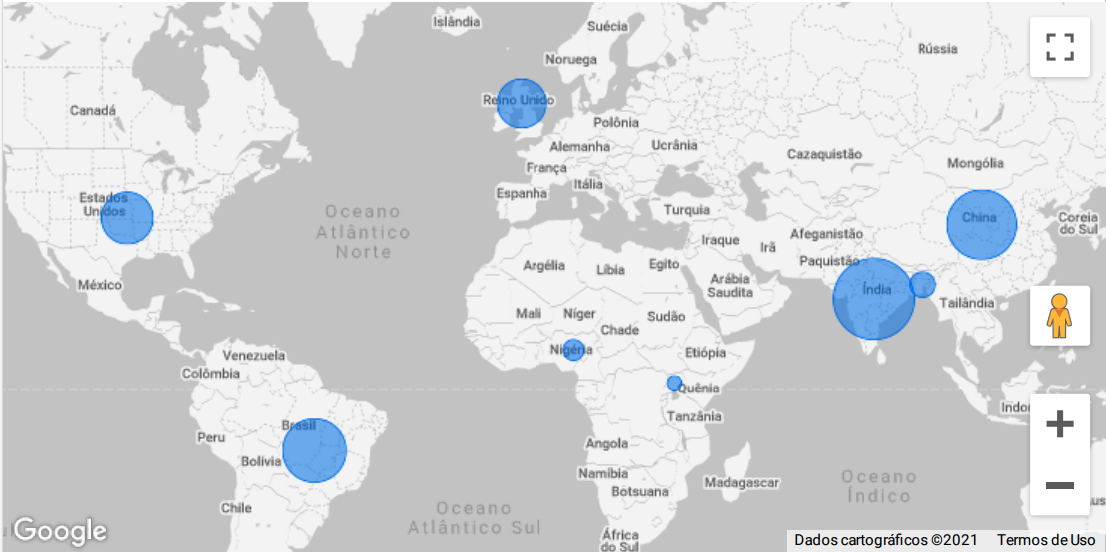
\includegraphics[width=1\textwidth]{img/met/map.png}
\caption{Mapa de Distribuição de Contas Coletadas}
\label{fig:map}
\end{figure}

A coleta dos usuários pela \emph{query} foi feita com o objetivo de ter os \emph{logins} dos usuários de interesse, para que seja possível a coleta de objetos específicos das ações deles, como os repositórios que colaboraram, os \emph{pull requests} feitos, as colaborações e as \emph{issues} criadas. 

Assim, foi desenvolvido outro código python com o objetivo de capturar os dados de cada repositório contribuído, \emph{pull request} participado e  \emph{issues} criada de cada \emph{login} coletado, representando os oito países em análises. Esses dados foram os utilizados para basear a discussão em relação as três perguntas definidas.

Nas Tabelas \ref{table:avg} e \ref{table:std}, respectivamente, são apresentados os valores médios e de desvio padrão da base de dados de cada país de estudo.

\begin{table}[ht]
\centering
\caption{Média dos atributos coletados por usuário}
\begin{tabular}{|c|c|c|c|c|c|}
\hline
País        & Comentários & Issues & PullRequests & \begin{tabular}[c]{@{}c@{}}Repositórios\\  contribuídos\end{tabular} & Seguidores \\ \hline
Estados Unidos  & 11,56          & 65,16  & 86,10        & 6,22                      & 78,72     \\ \hline
Reino Unido & 11,47          & 73,12  & 98,93        & 6,97                      & 76,36     \\ \hline
China       & 3,33           & 32,07  & 33,68        & 3,80                      & 176,25    \\ \hline
Brasil      & 2,95           & 21,38  & 30,04        & 3,58                      & 57,05     \\ \hline
Índia       & 1,58           & 17,39  & 23,75        & 3,83                      & 32,86     \\ \hline
Bangladesh  & 0,15           & 1,82   & 3,24         & 0,71                      & 4,68      \\ \hline
Nigéria     & 0,27           & 2,81   & 17,80        & 1,77                      & 5,77      \\ \hline
Uganda      & 0,94           & 5,80   & 37,57        & 2,12                      & 5,81      \\ \hline
\end{tabular}
\label{table:avg}
\end{table}

\begin{table}[ht]
\centering
\caption{Desvio Padrão dos atributos coletados por usuário}
\begin{tabular}{|c|c|c|c|c|c|}
\hline
País        & Comentários & Issues & PullRequests & \begin{tabular}[c]{@{}c@{}}Repositórios\\  contribuídos\end{tabular} & Seguidores \\ \hline
Estados Unidos & 81,19          & 182,79 & 308,20       & 23,22                     & 732,59    \\ \hline
Reino Unido    & 56,48          & 200,58 & 282,46       & 28,61                     & 532,71    \\ \hline
China          & 23,37          & 103,19 & 117,07       & 10,96                     & 1060,99   \\ \hline
Brasil         & 31,94          & 73,39  & 87,97        & 10,56                     & 281,73    \\ \hline
Índia          & 13,92          & 426,00 & 71,64        & 9,77                      & 131,90    \\ \hline
Bangladesh     & 0,96           & 9,75   & 15,09        & 2,66                      & 2,18      \\ \hline
Nigéria         & 1,48           & 10,15  & 43,39        & 4,55                      & 1,84      \\ \hline
Uganda         & 5,50           & 17,56  & 64,10        & 4,87                      & 1,85      \\ \hline
\end{tabular}
\label{table:std}
\end{table}

\section{Resultados} \label{sec:results}

\subsection{RQ1: Existe diferença entre as tecnologias mais utilizadas pelos países países com diferentes faixas de desenvolvimento?}

Para analisar a representatividade das linguagens que os usuários de cada país utilizavam, foram utilizados os dados de todos os repositórios que os usuários tiveram alguma contribuição no código. Para cada objeto de repositório coletado foi possível identificar o valor no campo \emph{language}, que representa a linguagem predominante identificada naquele repositório. Quando não é possível identificar uma linguagem de programação principal o campo é definido por \emph{Undefined language}.

No total, foram coletados 337.812 repositórios, dos 77.985 usuários da base de dados original, tendo então uma média de 7,29 repositórios por usuário. Nestes repositórios, foram identificadas 330 linguagens de programação diferentes, sendo que nos Estados Unidos e Reino Unido, representantes da faixa de IDH mais alta, foi possível identificar 242 e 236 linguagens diferentes, enquanto na Nigéria e Uganda, foram encontradas 54 e 31 linguagens diferentes.

A Figura \ref{fig:graphlanguages} permite uma visão geral sobre as diferenças entre a representatividade das linguagens em cada país, separados pela faixa de desenvolvimento que representam.

\begin{figure}[ht]
\centering
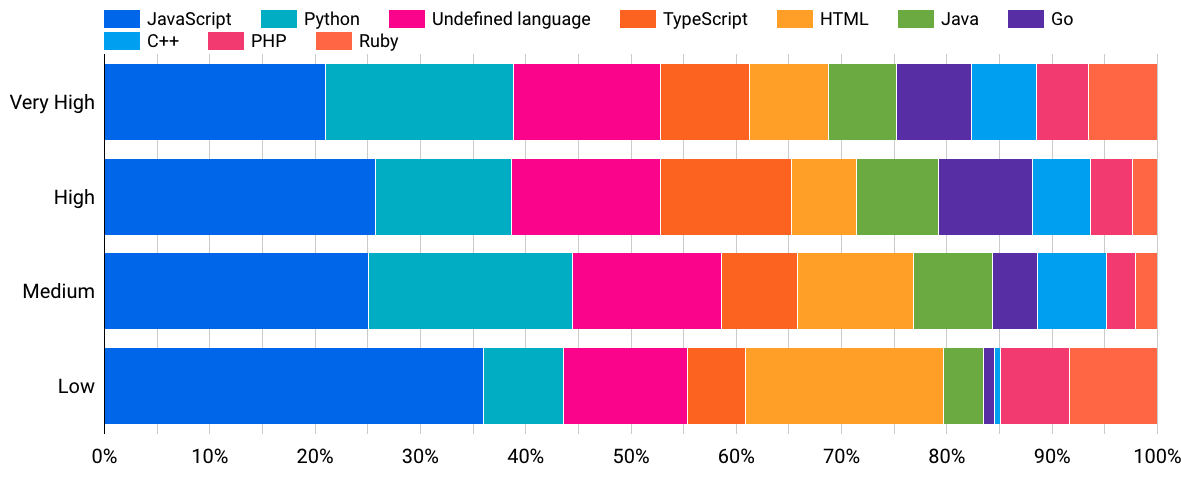
\includegraphics[width=1\textwidth]{img/rq1/graph_languages.png}
\caption{Representação de Linguagens por Faixa de IDH}
\label{fig:graphlanguages}
\end{figure}

Entretanto, para ter uma visão mais detalhada das diferenças entre as linguagens foco da pesquisa, é necessário a criação de gráficos específicos. Inicialmente, um dos nossos focos era a diferenciação entre a representatividade de linguagens usualmente utilizadas na área de ciência de dados, como Python e R. 

Em relação comparação da representatividade da linguagem Python, que pode ser observada na Figura \ref{fig:python}, temos que em forma geral o Python representa a linguagem de pelo menos 12\% dos repositórios coletados, com esse valor variando em cada país. Nessa linguagem, é notável um destaque para a Índia que apresenta a representatividade maior que 15\%. De forma geral, há uma tendência de diminuição da representatividade do Python com a diminuição do índice de desenvolvimento humano.

\begin{figure}[H]
\centering
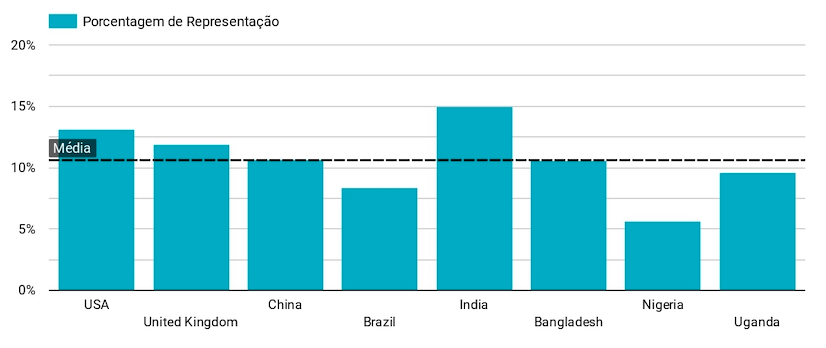
\includegraphics[width=1\textwidth]{img/rq1/python.png}
\caption{Representação da Linguagem Python}
\label{fig:python}
\end{figure}

Em relação a outra linguagem muito utilizada para ciência de dados, o R, temos na Figura \ref{fig:r}, apesar de números absolutos menores que o Python, quando comparada a representatividade, há um destaque  grande para os valores encontrados nos Estados Unidos e Reino Unido, representantes do IDH Muito Alto, em relação aos demais países. 

\begin{figure}[H]
\centering
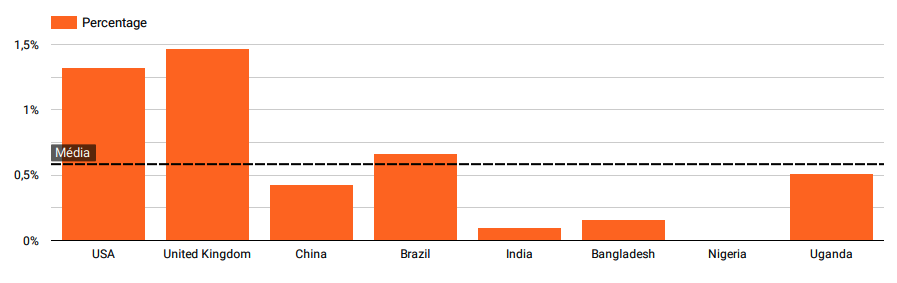
\includegraphics[width=1\textwidth]{img/rq1/r.png}
\caption{Representação da Linguagem R}
\label{fig:r}
\end{figure}

Em relação as linguagens base de desenvolvimento web, foram analisadas as representatividades das linguagens PHP e HTML, respectivamente nas figuras \ref{fig:php} e \ref{fig:html}. Na Figura \ref{fig:php} é possível destacar a grande representatividade de PHP no desenvolvimento em Bangladesh, que apresenta um número acima da média junto a Nigéria. Já em relação ao HTML, na Figura \ref{fig:html} temos que a Nigéria é o país com maior representatividade nessa linguagem, seguida por Uganda e Bangladesh, sendo os três países com menor índice de desenvolvimento da base considerada.

\begin{figure}[H]
\centering
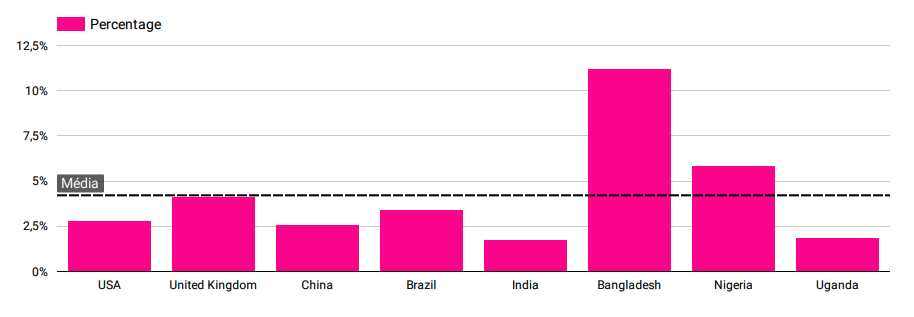
\includegraphics[width=1\textwidth]{img/rq1/php.png}
\caption{Representação da Linguagem PHP}
\label{fig:php}
\end{figure}

\begin{figure}[H]
\centering
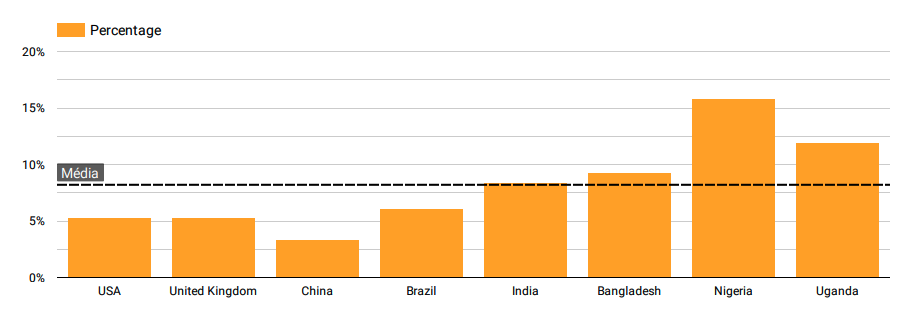
\includegraphics[width=1\textwidth]{img/rq1/html.png}
\caption{Representação da Linguagem HTML}
\label{fig:html}
\end{figure}

Uma linguagem que não estava inicialmente no foco da pesquisa mas que chamou a atenção pela diferença entre as representatividades é a linguagem Go. Temos que quase 10\% dos repositórios contribuídos pelos usuários chineses analisados eram da linguagem Go, e em exceção da China, os países com maiores índices de desenvolvimento tendem a ter maior representatividade da linguagem que os de menor.

\begin{figure}[H]
\centering
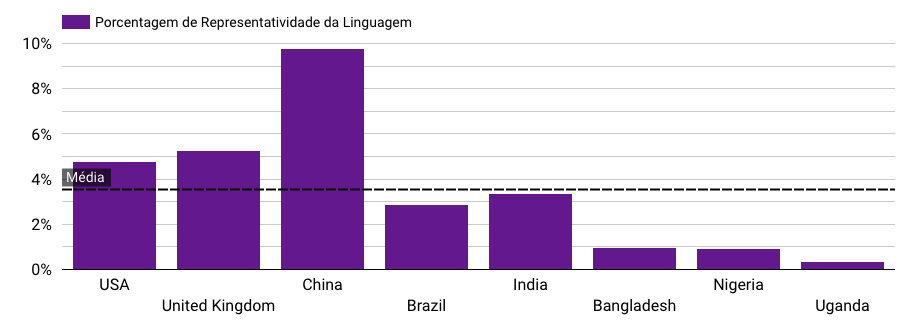
\includegraphics[width=1\textwidth]{img/rq1/go.png}
\caption{Representação da Linguagem Go}
\label{fig:go}
\end{figure}


\subsection{RQ2 - Existe uma diferença entre a tendência de contribuição em repositórios de código aberto de países com diferentes categorias de desenvolvimento?}

Para identificar a tendência de contribuição em repositórios de código aberto, foi utilizado também a base de dados dos 337.812 repositórios que representa todos os repositórios públicos que os 77.985 usuários dos oito países em análise contribuíram. 

A primeira métrica definida foi a porcentagem dos repositórios listados que se enquadram como repositórios populares, ou seja, com mais de 1.000 estrelas. Analisando a média geral da base de dados de repositórios coletados, temos que 18\% podem ser considerados repositórios populares, sendo que essa representatividade varia por país. Na Figura \ref{fig:porcpop}, é possível destacar que a China apresenta 27,54\% dos seus repositórios públicos contribuídos como repositórios populares, sendo um valor consideravelmente acima da média. Também é possível notar que Uganda, Nigéria e Brasil são os países com menor representatividade de repositórios populares

\begin{figure}[H]
\centering
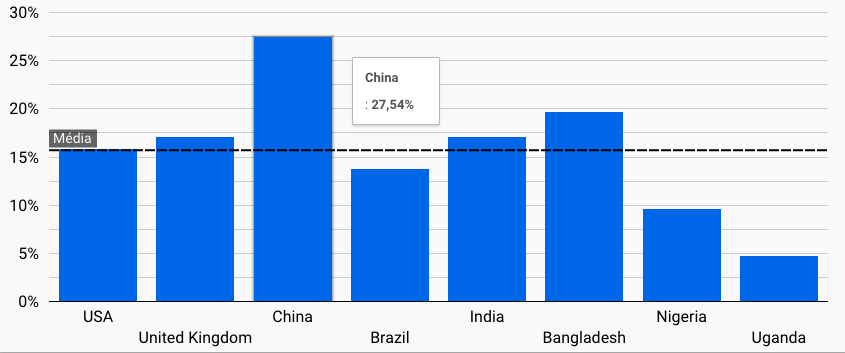
\includegraphics[width=1\textwidth]{img/rq2/porcpop.png}
\caption{Porcentagem de Repositórios Populares}
\label{fig:porcpop}
\end{figure}

A segunda métrica analisada foi a porcentagem de usuários que tem pelo menos uma contribuição em um repositório popular, ou seja a representatividade de usuários que pelo menos uma vez contribuíram para repositórios com mais de 1.000 estrelas. Na Tabela \ref{table:atleatone}, é possível identificar a porcentagem de usuários com contribuição em pelo menos um repositório popular de cada país.

\begin{table}[ht]
\centering
\caption{Usuários que contribuíram com pelo menos um repositório popular}
\begin{tabular}{|c|c|c|c|c|c|}
\hline
País        & Número de Usuários &  \begin{tabular}[c]{@{}c@{}}Número de Usuários\\ que contribuíram\\  para pelo menos um \\repositório popular\end{tabular} & \begin{tabular}[c]{@{}c@{}}Porcentagem de Usuários\\ que contribuíram\\  para pelo menos \\um repositório popular\end{tabular} \\ \hline
Estados Unidos & 7.173          & 3.715  & 51,79\% \\ \hline
Reino Unido    & 7.221          & 4.101  & 56,79\% \\ \hline
China          & 9.295          & 6.048  & 65,07\% \\ \hline
Brasil         & 9.088          & 3.266  & 35,64\% \\ \hline
Índia          & 11.519         & 5.235  & 45,45\% \\ \hline
Bangladesh     & 933            & 276    & 29,93\% \\ \hline
Nigéria         & 1.057         & 240    & 22,71\% \\ \hline
Uganda         & 135            & 24     & 17,78\% \\ \hline
\end{tabular}
\label{table:atleatone}
\end{table}

Na Figura \ref{fig:atleatone}, temos um opção mais visual de comparações entre esses números onde é possível notar o destaque da China, que tem grande parte dos seus usuários avaliados (65,07\%) no estudo contribuindo em repositórios populares.Temos que em exceção da China, que apresenta a maior porcentagem, e o Brasil, que tem uma porcentagem menor que da Índia, todos os demais países seguem a tendência de quanto maior o IDH maios a porcentagem de usuários contribuições em repositórios populares.

\begin{figure}[H]
\centering
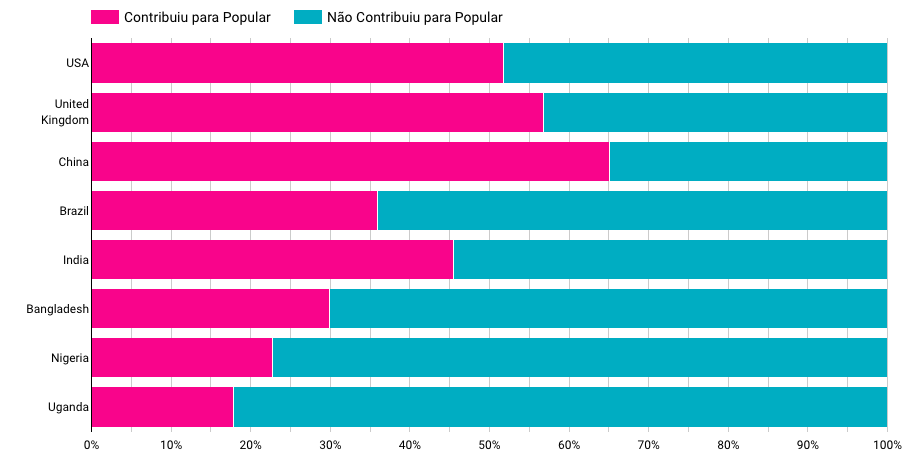
\includegraphics[width=1\textwidth]{img/rq2/atleatone.png}
\caption{Usuários que contribuíram com pelo menos um repositório popular}
\label{fig:atleatone}
\end{figure}

A terceira métrica em relação a contribuição em repositórios populares analisadas foi, a quantidade média de repositórios populares contribuídos por usuário. Esse número representa, portanto, quantos repositórios públicos em média cada usuário contribui e quantos desses são repositórios populares, como mostra na Tabela \ref{table:avgpop}

\begin{table}[ht]
\centering
\caption{Usuários que contribuíram com pelo menos um repositório popular}
\begin{tabular}{|c|c|c|c|c|c|}
\hline
País        & \begin{tabular}[c]{@{}c@{}}Valor médio de \\repositórios \\contribuídos\end{tabular} &  \begin{tabular}[c]{@{}c@{}}Valor médio de \\repositórios populares \\contribuídos \end{tabular} & \begin{tabular}[c]{@{}c@{}}Porcentagem média de \\repositórios populares\\ contribuídos\end{tabular} \\ \hline
Estados Unidos & 9,67          & 1,54  & 20.57\% \\ \hline
Reino Unido    & 9,94          & 1,71  & 22,50\% \\ \hline
China          & 6,65          & 1,83  & 35,02\% \\ \hline
Brasil         & 5,74          & 0,79  & 15,35\% \\ \hline
Índia          & 6,58          & 1,12  & 19,30\% \\ \hline
Bangladesh     & 2,66          & 0,52  & 18,33\% \\ \hline
Nigéria        & 3,57          & 0,35  & 11,09\% \\ \hline
Uganda         & 4,33          & 0,21  & 9,94\%  \\ \hline
\end{tabular}
\label{table:avgpop}
\end{table}

Para uma análise visual comparativa, temos na Figura \ref{fig:avgpop} que a China mantém uma porcentagem maior que os demais países, e que os países de faixa de IDH considerada baixa, Nigéria e Uganda, tem a menor representatividade de repositórios populares entre os repositórios contribuídos por usuário.

\begin{figure}[H]
\centering
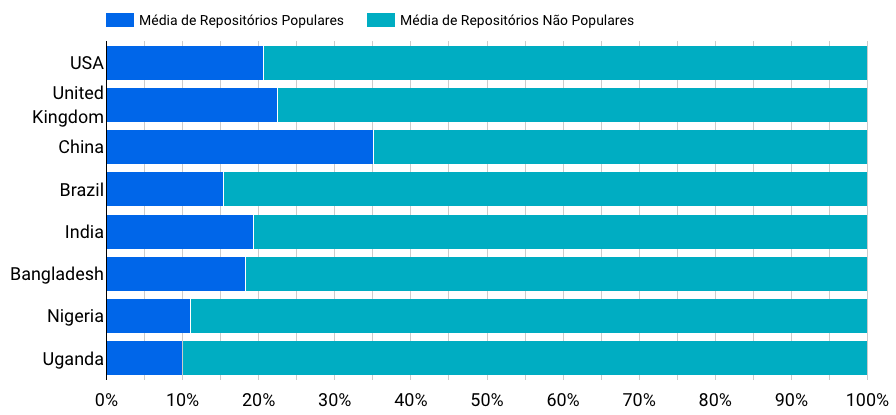
\includegraphics[width=1\textwidth]{img/rq2/avgpop.png}
\caption{Média repositórios populares contribuídos por usuário}
\label{fig:avgpop}
\end{figure}

\subsection{RQ3 - Existe uma diferença entre os hábitos de desenvolvimento de países com diferentes categorias de desenvolvimento?}

Para identificar os hábitos de desenvolvimento, foram analisadas uma base contendo 1.046.026 PRs e outra com 603.658 Issues nos quais foram originados pelos 77.985 usuários dos oito países em análise. Vale ressaltar que destes 77.985 usuários apenas 39.185 criaram ao menos uma \textit{Issue} e, no mesmo sentido, apenas 60.007 usuários criaram ao menos um \textit{PR}.

Como primeira métrica, decidimos obter a quantidade de \textit{Pull Requests} de cada país. Na Figura \ref{fig:qttprs}, temos a distribuição dos \textit{Pull Requests} pelos países em análise. Em destaque, nota-se a grande representatividade dos países do bloco de IDH 'Muito Alto', representando 41,71\% do total com 436.310 \textit{PRs} originados pelos países, com uma média de cerca de 12 \textit{PRs} por usuário deste bloco. Outro ponto de destaque é a Índia, que, sozinha, possui quase a mesma quantidade de \textit{Pull Requests} do Reino Unido(que é um conjunto de países) e ultrapassa a média do bloco citado com uma média de 14 \textit{PRs} por usuário.

\begin{figure}[!htb]
\centering
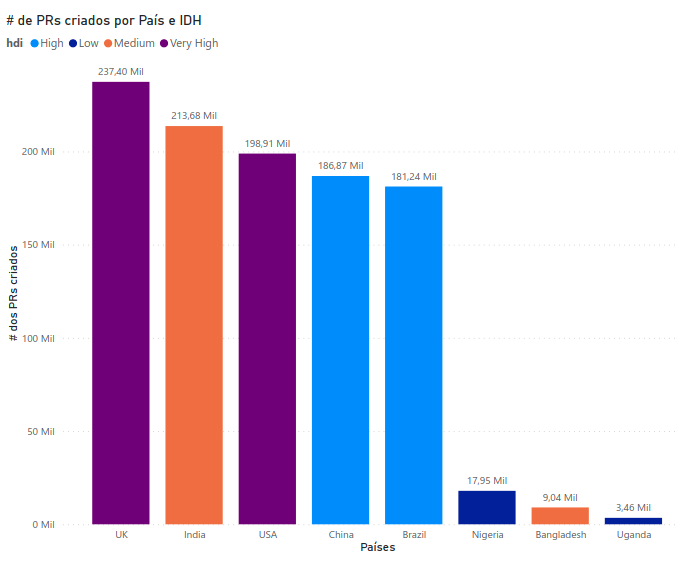
\includegraphics[width=1\textwidth]{img/rq3/number of prs.png}
\caption{Quantidade de PULL REQUESTs criados por país}
\label{fig:qttprs}
\end{figure}

A segunda métrica analisada foi a duração dos PRs em cada país. Para isso calculamos a média e a mediana da duração dos em horas. Como resultado inicial, o país que leva mais tempo na média para concluir um PR é a China com cerca 281 horas conforme a Figura \ref{fig:media_prs}, seguido do Brazil, seu companheiro de bloco de IDH, com 244 horas. Com isso teríamos que, em média a China avalia um PR em cerca de 11 dias e o Brasil 24, enquanto que os países do bloco 'Baixo' levam cerca de 4 dias na avaliação. 

\begin{figure}[H]
\centering
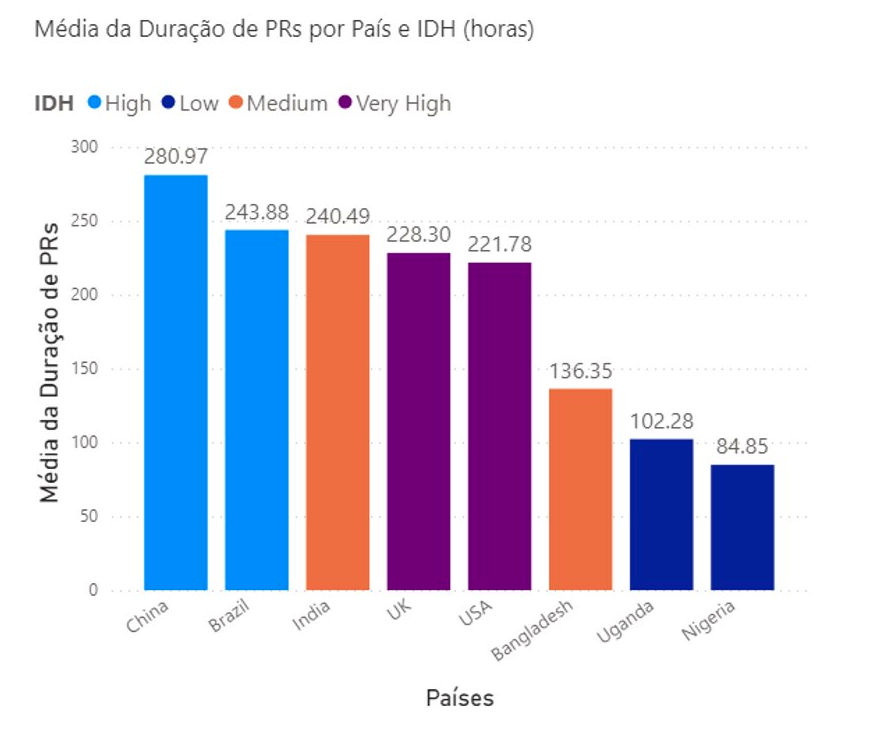
\includegraphics[width=1\textwidth]{img/rq3/media pr.png}
\caption{Média do tempo de avaliação de um PULL REQUEST por país}
\label{fig:media_prs}
\end{figure}

Verificando agora a mediana temos um empate entre a China, Reino Unido e Estados Unidos com duas horas, a Índia com uma hora e o restante dos países levando menos de uma hora para realizar a avaliação conforme mostra a Figura \ref{fig:mediana_prs}.

\begin{figure}[H]
\centering
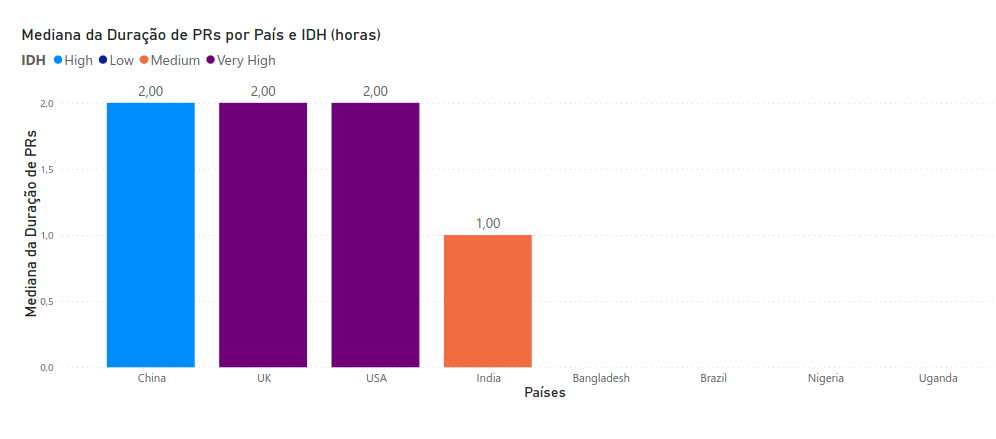
\includegraphics[width=1\textwidth]{img/rq3/mediana prs.png}
\caption{Mediana do tempo de avaliação de um PULL REQUEST por país}
\label{fig:mediana_prs}
\end{figure}

Avaliando a terceira métrica, o número médio de linhas alteradas por commit por país, temos, na Figura \ref{fig:media_linhas} um destaque para os países desenvolvidos é que estes alteram menas linhas de código por commit, com exceção da China que, na média, altera mais linhas que a Índia em seus commits.

\begin{figure}[H]
\centering
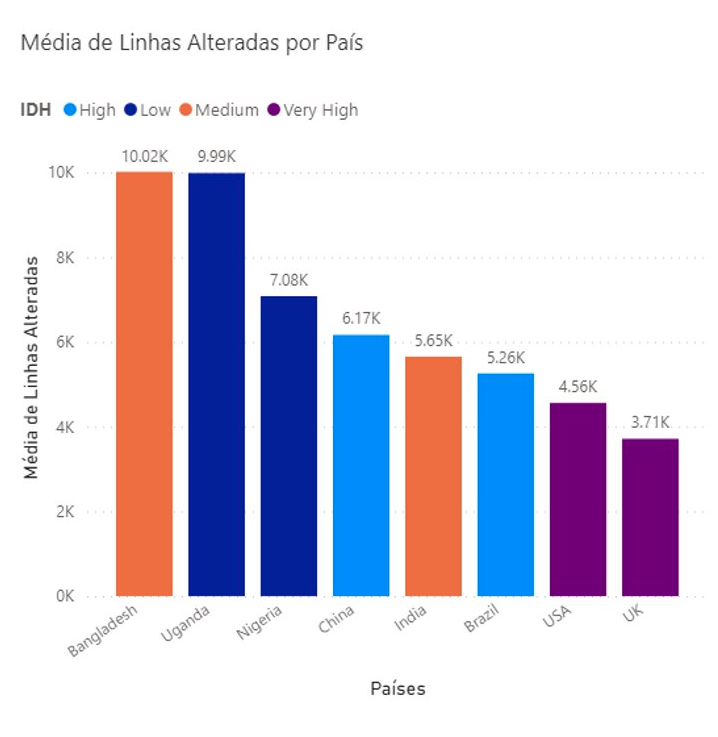
\includegraphics[width=0.7\textwidth]{img/rq3/media linhas.png}
\caption{Média de linhas alteradas por COMMIT por país}
\label{fig:media_linhas}
\end{figure}

Considerando novamente a mediana, a Figura \ref{fig:medianalinhas} redefine o \textit{ranking},  mantendo apenas os países menos desenvolvidos seguindo a média com a Uganda alterando 121 linhas e a Nigéria 95 na mediana. Observa-se ainda um padrão entre a China, Reino Unido e Estados Unidos, todos em torno de 36 linhas alteradas por commit, considerando a mediana.

\begin{figure}[H]
\centering
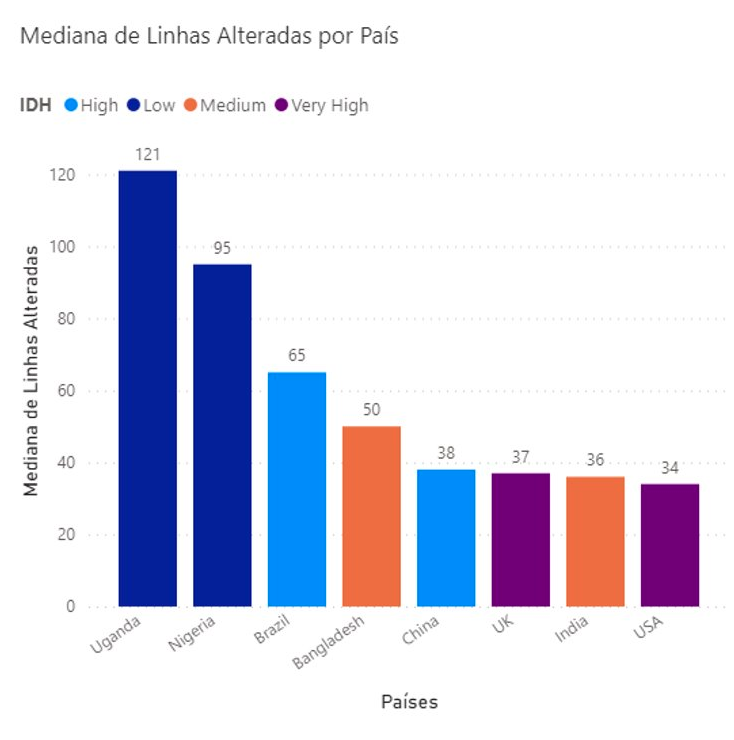
\includegraphics[width=1\textwidth]{img/rq3/mediana linhas.png}
\caption{Mediana de linhas alteradas por COMMIT por país}
\label{fig:medianalinhas}
\end{figure}

A quarta métrica muda o foco dos \textit{Pull Requests} para as \textit{Issues} criadas pelos países. Na figura \ref{fig:qttissues}, temos que a Índia se mostra como tendo os usuários que mais criam \textit{Issues} nos repositórios \textit{open source}, porém a diferença entre ela os Estados Unidos e Reino Unido é pequena. O Brasil cria menos da metade das \textit{Issues} em relação a Índia, e os números da Nigéria, Bangladesh e Uganda se mostram inexpressivos perantes aos outros sendo que juntos somam um total de 0,87\% do total das \textit{issues} criadas.

\begin{figure}[H]
\centering
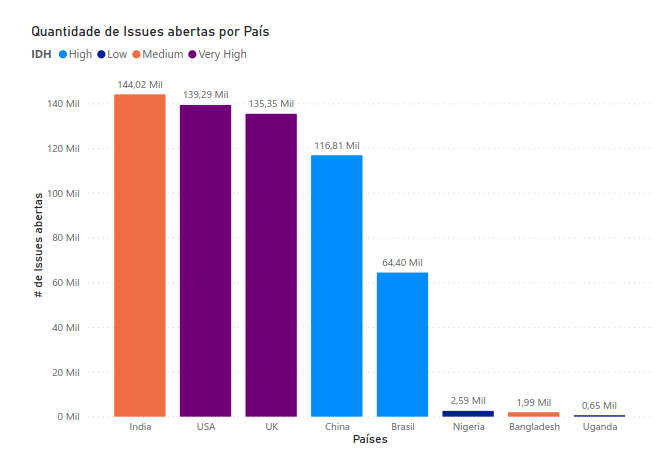
\includegraphics[width=1\textwidth]{img/rq3/number of issues.png}
\caption{Quantidade de ISSUEs abertas por país}
\label{fig:qttissues}
\end{figure}

Analisando ainda as \textit{Issues}, calculamos a média de duração e o resultado pode ser conferido na Figura \ref{fig:media_issue}. \textit{Issues} criadas pelo Reino Unido e Estados Unidos tendem a ser as que mais demoram a ser fechadas. Percebe-se que conforme diminui o nível de IDH, diminui também o tempo médio de duração das \textit{Issues}.



\begin{figure}[H]
\centering
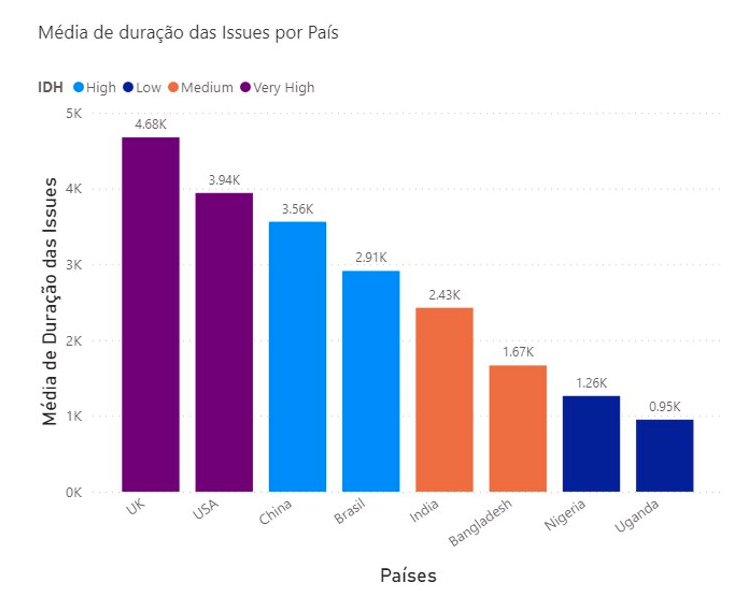
\includegraphics[width=1\textwidth]{img/rq3/media dur issues.png}
\caption{Média do tempo que se leva para fechar uma ISSUE por país}
\label{fig:media_issue}
\end{figure}

O gráfico da Figura \ref{fig:mediana_issue} considera a mediana da de duração das \textit{Issues}. Neste caso, a única mudança na relação entre os países foi que Bangladesh passa a ser o país que cria as issues que são concluídas mais rapidamente.

\begin{figure}[H]
\centering
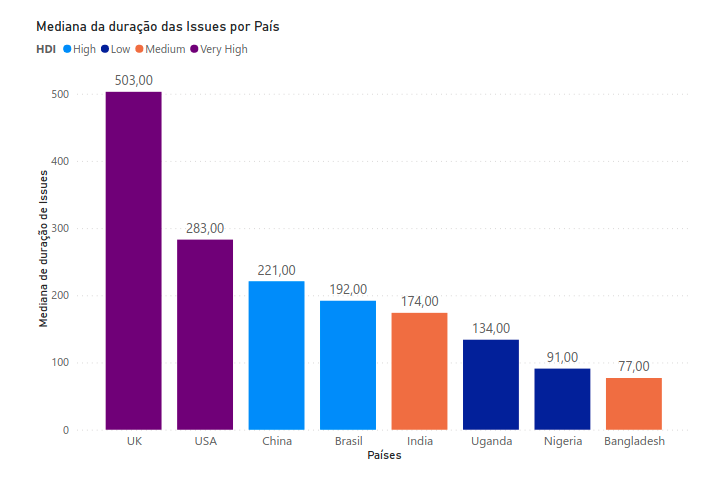
\includegraphics[width=1\textwidth]{img/rq3/mediana issues.png}
\caption{Mediana do tempo que se leva para fechar uma ISSUE por país}
\label{fig:mediana_issue}
\end{figure}

\section{Discussão} \label{sec:discussion}

Referente a análise dos resultados obtidos nos dados das linguagens utilizadas em cada país, podemos observar tendências gerais, relacionadas ao índice de desenvolvimento dos países, e destaques individuais. De maneira geral, é possível observar que os países de faixa de IDH considerada como ``Muito Alto'', costumam apresentar uma representatividade acima da média em linguagens utilizadas na área de ciência de dados, como o Python e o R. Para faixas de ``Alto'' e inferiores, a diferença não parece tão expressiva entre os demais países. Dentro dessas linguagens analisadas, destaca-se a exceção para representação do Python na Índia, que representa 15\% de todos os repositório contribuídos pela base de usuários indiana analisada, sendo um país de faixa de IDH ``Média''.

Por outro lado, é possível comparar também que os países de faixa de IDH ``Baixa'', são os com maior a representatividade de linguagens \textit{web} base como HTML, com destaque à Nigéria. Em relação ao PHP, os países com maior representatividade da linguagem são Bangladesh e Nigéria, respectivamente das faixas de IDH ``Médio'' e ``Baixo'', sendo que Bangladesh o PHP representa 13,84\% dos repositórios totais coletados.

Outra linguagem que apresentou um comportamento de destaque foi o Go, que apresenta uma tendencia de quanto maior o IDH maior a representatividade, entretanto com exceção da China, que tem cerca de 13,51\% dos repositórios coletados identificados na linguagem Go. 

Em relação a análise da contribuição em repositórios populares, temos que há sempre um destaque grande da China em relação tanto a representatividade dos repositórios populares contribuídos em relação aos repositórios totais, quanto a contribuição única ou constante por usuário nesses repositórios. Junto a isso, o destaque inicial na análise da base de dados de usuários, que mostra que usuários da China tem uma tendência muito maior de ter maior número de seguidores, mostra que a China aparenta ter uma tendência maior de utilizar o \textit{GitHub} realmente como uma rede social para o desenvolvimento, com mais colaboração e vinculação entre os usuários.

Desconsiderando a peculiaridade da China, os demais países seguem a tendência de quanto maior o Índice de Desenvolvimento Humano, maior a representatividade de repositórios populares entre os contribuídos pelos usuários. O único país que apresenta valores médios abaixo do esperado pela sua faixa de IDH é o Brasil, que tanto para a representatividade geral de repositórios populares contribuídos quanto para a média da porcentagem de repositórios populares por usuário, tem valores menores que dos países de faixa ``Média''. 

Quanto aos hábitos de desenvolvimento, os países compreendidos no bloco de IDH "Muito Alto" demonstram uma tendência em estar entre os, se não os, mais bem colocados em todas as comparações realizadas neste estudo. Das comparações realizadas, apenas a comparação quanto a duração do tratamento das \textit{Issues} seguiu um padrão do nível de IDH de forma expressiva. Como verificado na seção de resultados, nas Figuras 18 e 19, quanto menor o nível de IDH, menor é o tempo em média que se leva para tratar o problema levantado no repositório. Isso pode demonstrar que os desenvolvedores dos países mais desenvolvidos estão mais envolvidos com a comunidade open-source e criam \textit{Issues} sobre assuntos mais complexos e acabam demandando mais tempo para avaliação.

De forma geral, a Índia se destacou em vários aspectos dos hábitos de desenvolvimento demonstrando médias e medianas melhores do que os países dos blocos acima, principalmente em comparação ao Brasil. Na criação de \textit{Issues} e \textit{Pull Requests} a Índia aparece entre os primeiros em termos absolutos, porém quando trazemos para o âmbito da média por usuário, sua superioridade se mantêm apenas quanto aos \textit{Pull Requests} com 14 por usuário em média, enquanto que nas criações de \textit{Issues} teve apenas 16 por usuário superada pelos EUA com 21 e pelos UK com 20. Enquanto isso, o outro país do bloco 'Médio', o Bangladesh, se destoa completamente da Índia em todos os aspectos avaliados. Em algumas características, Bangladesh se torna o divisores entre os quatro países mais desenvolvidos e os menos desenvolvidos.

Analisando os resultados dos países do bloco 'Alto', temos que houve um destaque na média de duração dos PRs com 281 horas para a China e 244 horas para o Brasil, correspondendo a 11 e 10 dias respectivamente. Mesmo este bloco se mostrando os que teriam uma maior média de tempo para avaliação dos PRs criados, ao avaliar a mediana temos um empate técnico entre todos os países sendo que os valores ficaram num intervalo de 'menos de uma hora' e 2 horas.  

Os países com IDH 'Baixo' demostram resultados, no geral, inferiores aos usuários dos outros blocos. Porém é necessário considerar que a base de usuários identificados como desses países é significativamente menor que a base dos outros países. Por exemplo, Uganda e Nigéria são os países que mais alteram linhas por \textit{commit}, o que pode demostrar que os usuários destes países têm pouca vivência no sentido de que um \textit{commit} / \textit{pull request} deveria ser atômico.

% \textcolor{red}{Diante dos dados coletados nesta pesquisa e seguindo os gráficos apresentados podemos fazer uma relação dos dados de XXXX, levando em conta a não normalização dos dados (Ou normalização, usando o parâmetro YYYYY) e a relação dos dados coletados sendo 10\% da massa de usuários do total de cada país elencado. Consideramos que XXXX.}

\section{Ameaças à Validade} \label{sec:threatstovalidity}

Algumas das restrições do projeto são destacadas nesta seção a fim de evidenciar algumas ameaças à validade do estudo proposto, dentre elas podemos citar que:  

1 - Não há no \textit{GitHub} a disponibilização dos dados acerca da localização dos \textit{users}, por ser um campo aberto para permitir aos usuários mascarar a sua localização real. Dessa forma, mesmo aplicando o filtro de busca com base na localização os usuários coletados podem não corresponder à realidade.

2 - A seleção de poucos países e uso dos dados públicos disponibilizados pelo GitHub, foi selecionado apenas uma amostra estratificada da população, de forma que pode haver uma maior representatividade daquele país em outra ferramenta que não foi abordada neste trabalho.

3 - Em um país específico, o caso da Índia foi preciso fazer uma alteração na busca dado às restrições da API. Foi necessário manipular os dados para coletar. O uso de siglas, de cada país, foi necessário remover a expressão ´IN' pois a interface disponibilizada utiliza um método de contém, verificando se em toda a expressão escolhida há o texto, em parte pelo menos do parâmetro informado. Dessa forma foi preciso remover tal expressão pois dados incoerentes estavam sendo retornados.

4 - O \textit{GitHub}, apesar de ser uma das principais fontes de dados para comportamentos de desenvolvimento, não é a única, representando apenas uma parte da comunidade de desenvolvimento de cada país. Além disso, a utilização mais frequente do \textit{GitHub} ou de outro sistema pode sofrer influência dos hábitos de desenvolvimento do país, afetando a pesquisa.

5 - Dentro dos objetos de ações de desenvolvimento capturados pela API do \textit{GitHub}, temos acesso apenas aos realizados em repositórios públicos. Isso limita os dados que foram analisados, já que uma grande parte do desenvolvimento é feito em repositórios privados.

6 - Devido as limitações da API expostas, a pesquisa foi feita com a base de dados dos 10\% dos usuários identificados com maior número de seguidores de cada país. Essa amostra especifica, pode auxiliar na pesquisa, de forma que os usuários com maior número de seguidores tendem a ser os mais ativos, porém também poderia contaminar a base de usuários de algum país.

\section{Conclusão} \label{sec:conclusion}
Após a exposição dos dados coletados e a discussão levantada com base nos achados podemos concluir que há uma tendência de países de desenvolvimento ``Muito Alto'' terem uma maior representatividade de contribuições em linguagens de ciência de dados, como Python e R e países da faixa de IDH ``Baixa'' terem maiores contribuições para repositórios em linguagens web básicas como PHP e HTML. Entretanto, não é possível generalizar em relação às demais faixas de desenvolvimento. Como pontos de destaques nas linguagens temos a Índia com Python, Bangladesh com PHP e Nigéria com HTML.

Além disso, concluímos que a China apresenta um comportamento, no \textit{GitHub}, de colaboração e vinculação entre os usuários, com os maiores números de seguidores e contribuições em repositórios populares, de forma geral e por usuário. Em relação a contribuição dos usuários, concluímos também que há a tendência de quanto maior o IDH, maior a representação de repositórios populares entre os contribuídos, com exceção da China, que apresenta um valor que extrapô-la o esperado, e o Brasil, que apresenta um valor abaixo do esperado.

Com relação aos hábitos técnicos de criação e atividades relacionadas aos \textit{Pull Requests} e \textit{Issues}, nota-se que os países mais desenvolvidos possuem uma tendência em ser mais ativos e trazer contribuições possivelmente mais relevantes quanto às métricas estudadas dado que a duração de ambos é maior quanto maior o nível de IDH do país daquele desenvolvedor que criou o  \textit{PR/Issue}. 

Concluímos também que apesar de que a Índia ter apresentado números absolutos grandes em comparação aos outros países quanto a elaboração de \textit{Pull Requests} e \textit{Issues}, ao analisarmos a média por usuário, por exemplo, se mostra inferior aos países com maior IDH. Num contexto geral dos dados analisados, pôde-se observar que quando separados por IDH as diferenças e tendências acompanham a diminuição / aumento no nível de IDH do país em questão, salvo algumas exceções como a mediana de linhas alteradas por \textit{commit}. 

Como trabalho futuro e visando criar uma maior assertividade pode se expandir a coleta para os 25\% de usuários mais representativos a fim de coletar o primeiro quartil amostral da população. Além disso, seria possível realizar uma busca mais profunda em relação ao real número disponível de usuários de cada país ou a realização de um trabalho com um grupo maior de países em estudo.

\bibliographystyle{sbc}
\bibliography{sbc-template}

\end{document}
